% +--------------------------------------------------------------------+
% | LaTeX Template                                                     |
% | for K-State Electronic Theses, Dissertations, and Reports          |
% |                                                                    |
% | Comments and guidelines for using the template are shown           |
% | within boxes like this one.                                        |
% |                                                                    |
% | Revised 6/30/06                                                    |
% | 9/14/06: Removed typos                                             |
% +--------------------------------------------------------------------+

\documentclass[final, 12pt,oneside]{class_diss}

\usepackage[utf8]{inputenc}
\usepackage[T1]{fontenc}
\usepackage[spanish]{babel}
% +--------------------------------------------------------------------+
% | Now, we add in all external packages that we will use throughout   |
% | the document.  You can add other packages as needed.
% +--------------------------------------------------------------------+

%\usepackage{     caption2} % Customize captions a bit more
\usepackage{      amsmath} % American Mathematics Society standards
%\usepackage{      wrapfig} % Wraps text around a figure or table
\usepackage{     graphicx} % Extended graphics package.
%\usepackage{     fancyhdr} % Efficiently handles headers and footers
%\usepackage{       braket} % Bra-Ket notation package
%\usepackage{     mathrsfs} % Specialized Math fonts (Hamiltonian, etc.)
%\usepackage{boxedminipage} % Boxed text can be produced
%\usepackage{     setspace} % Controls line spacing via \begin{space}

\usepackage{amsxtra}
\usepackage{amssymb}
\usepackage{amsthm}
\usepackage{latexsym}
\usepackage{listings}

% +--------------------------------------------------------------------+
% | The color package allows one to select colors for hyperlinking     |
% | (see below).                                                       |
% +--------------------------------------------------------------------+

\usepackage[usenames]{color}

% +--------------------------------------------------------------------+
% | Colors defined for use with this template.                         |
% +--------------------------------------------------------------------+

\definecolor{  Pink}{rgb}{1.0, 0.5, 0.5}
\definecolor{Maroon}{rgb}{0.8, 0.0, 0.0}

\usepackage[pdftex, plainpages=false, pdfpagelabels]{hyperref}

\hypersetup{
    linktocpage=true,
    colorlinks=true,
    bookmarks=true,
    citecolor=blue,
    urlcolor=red,
    linkcolor=Maroon,
    citebordercolor={1 0 0},
    urlbordercolor={1 0 0},
    linkbordercolor={.7 .8 .8},
    breaklinks=true,
    pdfpagelabels=true,
}

% +--------------------------------------------------------------------+
% | Page margins are set on 1 inch on all sides.                       |
% +--------------------------------------------------------------------+

\topmargin      = -0.56in
\textheight     =  8.60in
\textwidth      =  6.46in
\oddsidemargin  =  0.02in

% +--------------------------------------------------------------------+
% | The document finally begins here.                                  |
% +--------------------------------------------------------------------+
\begin{document}

  \setcounter{page}{-1}

% +--------------------------------------------------------------------+
% | Title Page
% +--------------------------------------------------------------------+
% +--------------------------------------------------------------------+
% | Title Page
% +--------------------------------------------------------------------+

\newpage

% +--------------------------------------------------------------------+
% | This page should not contain a page number.  We use the
% | \thispagestyle[empty] command below to suppress page numbers
% | and other style elements.
% +--------------------------------------------------------------------+

\thispagestyle{empty}

% +--------------------------------------------------------------------+
% | The Title page begins here.
% +--------------------------------------------------------------------+

\begin{center}

   \vspace{1cm}

   {\Large Predicción a corto plazo de la energía
   	 generada por una placa solar}\\

   \vspace{0.5cm}

   \vspace{0.5cm}

   {\large Pablo Aragón Moreno}\\
   {\large María Castañeda López}\\
   {\large Abel Coronado López}\\
 
   \vspace{0.5cm}

   GRADO EN INGENIERÍA INFORMÁTICA. FACULTAD DE INFORMÁTICA\\
   UNIVERSIDAD COMPLUTENSE DE MADRID \\


   \vspace{0.65cm}
   \rule{2in}{0.5pt}\\
   \vspace{0.85cm}

  
\includegraphics[height=2.5in]{figures/escudo.jpg}
  

   \vspace{0.5cm}
Trabajo Fin de Grado en Ingeniería Informática

   \vspace{0.5cm}

% +--------------------------------------------------------------------+
%  Fecha 
% +--------------------------------------------------------------------+

  26 de Junio de 2017\\
   \vspace{1cm}

\end{center}

{\raggedleft
Director/es y/o colaborador:\\
   \vspace{ 1cm}
José Ignacio Gómez\\
Christian Tenllado\\
}


% +--------------------------------------------------------------------+
% | Use the section below if you have co-major professors.
% +--------------------------------------------------------------------+

%\begin{flushleft}
%   \hspace{10cm}Approved by:\\
%   \vspace{ 1cm}
%   \hspace{10cm}Co-Major Professor\\
%   \hspace{10cm}Enter Your Co-Major Professor's Name\\
%   \vspace{.5cm}
%   \hspace{10cm}Co-Major Professor\\
%   \hspace{10cm}Enter Your Co-Major Professor's Name\\
%\end{flushleft}

   \pdfbookmark[0]{Portada}{PDFPortadaPage}

% +--------------------------------------------------------------------+
% | Authorizacion Page
% +--------------------------------------------------------------------+
% +--------------------------------------------------------------------+
% | Copyright Page
% +--------------------------------------------------------------------+

\newpage

\thispagestyle{empty}

\begin{center}

{\bf \Huge Autorización de difusión}

\vspace{1cm}

    {\large Pablo Aragón Moreno}\\
    {\large María Castañeda López}\\
    {\large Abel Coronado López}\\

   \vspace{0.5cm}

% +--------------------------------------------------------------------+
% | On the line below, replace Fecha
% |
% +--------------------------------------------------------------------+

   26 de Junio de 2017\\
   \vspace{0.5cm}

\end{center}
   
El/la abajo firmante, matriculado/a en el Grado en Ingeniería Informática de la Facultad de Informática, autoriza a la Universidad Complutense de Madrid (UCM) a difundir y utilizar con fines académicos, no comerciales y mencionando expresamente a su autor el presente Trabajo Fin de Grado: “Predicción a corto plazo de la energía
   	 generada por una placa solar”, realizado durante el curso académico 2016-2017 bajo la dirección de Jose Ignacio Gómez, y a la Biblioteca de la UCM a depositarlo en el Archivo Institucional E-Prints Complutense con el objeto de incrementar la difusión, uso e impacto del trabajo en Internet y garantizar su preservación y acceso a largo plazo.


   \pdfbookmark[0]{Autorización}{PDFAutorizacionPage}

   % +--------------------------------------------------------------------+
% | Copyright Page
% +--------------------------------------------------------------------+

\newpage

\thispagestyle{empty}

\begin{center}

{\bf \Huge Resumen en castellano}

  \end{center}
\vspace{1cm}

Proyecto que intenta predecir la radiación solar que habrá en un punto en un intervalo de tiempo definido utilizando modelos predictivos.

\vspace{1cm}

\begin{center}

{\bf \Large Palabras clave}
\vspace{1cm}

   Radiación solar
   \vspace{0.5cm}

   Placa solar
   \vspace{0.5cm}

   Raspberry Pi
   \vspace{0.5cm}

   Piranómetro
   \vspace{0.5cm}

   Inteligencia artifical
   \vspace{0.5cm}

   Algoritmos
   \vspace{0.5cm}

   Predicción
   \vspace{0.5cm}

   \end{center}

   \vspace{0.5cm}

   




   



   
   \pdfbookmark[0]{Resumen}{PDFResumenPage}

    % +--------------------------------------------------------------------+
% | Copyright Page
% +--------------------------------------------------------------------+

\newpage

\thispagestyle{empty}

\begin{center}

{\bf \Huge Abstract}

  \end{center}
\vspace{1cm}

Project that attempts to predict solar radiation at a point in a defined time interval using predictive models.

\vspace{1cm}

\begin{center}

{\bf \Large Keywords}
\vspace{1cm}

   Solar radiation
   \vspace{0.5cm}

   Solar panel
   \vspace{0.5cm}

   Raspberry Pi
   \vspace{0.5cm}

   Pyranometer
   \vspace{0.5cm}

   Machine learning
   \vspace{0.5cm}

   Algorithms
   \vspace{0.5cm}

   Prediction
   \vspace{0.5cm}

   \end{center}

   \vspace{0.5cm}
   



       \pdfbookmark[0]{Abstract}{PDFAbstractPage}
    \vfill

\newpage
\pagenumbering{roman}

\setcounter{page}{1}

\phantomsection
\addcontentsline{toc}{chapter}{Índice}

\tableofcontents

% +--------------------------------------------------------------------+
% | Acknowledgements Page
% +--------------------------------------------------------------------+
\newpage
\begin{center}
{\bf \Huge Agradecimientos}
\end{center}
\vspace{1cm}
\setlength{\baselineskip}{0.8cm}

A \textbf{Jose Ignacio Gómez} por su implicación, atención y paciencia. Siempre dispuesto a orientarnos a lo largo de todo el proyecto y de enseñarnos aquello que no conocíamos.


\phantomsection
\addcontentsline{toc}{chapter}{Agradecimientos}

\newpage
\pagenumbering{arabic}
\setcounter{page}{1}

% +--------------------------------------------------------------------+
% | Chapters
% +--------------------------------------------------------------------+
\cleardoublepage

\chapter{Introducción}
%\label{ch:chapter1}
\label{makereference}

Aquí haremos un breve resumen de la motivación y de la descripción del sistema.

\begin{figure}[htb]%t=top, b=bottom, h=here
	
	\begin{center}
		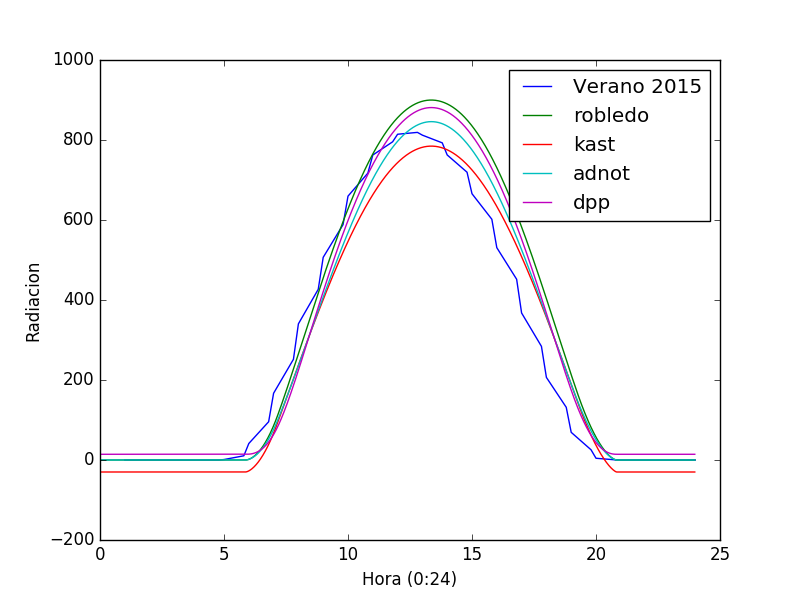
\includegraphics[height=2.5in]{figures/verano2015.png}
		\caption{Modelo verano 2015}
	\end{center}
    
    \label{figure1}
\end{figure}

% +--------------------------------------------------------------------+
% |To create cross-references to figures, tables and segments
% |of text, LaTeX provides the following commands:
% |   \label{marker}
% |   \ref{marker}
% |   \pageref{marker}
% | where {marker} is a unique identifier.
% |
% | In the line above, we use \label{figure1} to mark a location
% | we wish to refer to later.  LATEX replaces \ref by the number of
% | the chapter, section, subsection, figure, or table after which the
% | corresponding \label command was issued. \pageref prints the page
% | number of the page where the \label command occurred.
% |
% +--------------------------------------------------------------------+

Here is an example of a Table:

\begin{table}

% +--------------------------------------------------------------------+
% | We include the command \begin{center} to center the table
% | horizontally on the page.  Note use of the command \end{center}
% | to turn off centering after the table is defined.
% +--------------------------------------------------------------------+
    \begin{center}

% +--------------------------------------------------------------------+
% | The table is created with this command
% |
% | \begin{tabular}[pos]{table spec}
% |
% | The "pos" argument specifies the vertical position of the table relative to
% | the baseline of the surrounding text.  Use t, b, or c to specify alignment
% | at the top, bottom, or center.
% |
% | The "table spec" command defines the format of the table
% |   l for a column of left-aligned text
% |   r for a column of right-aligned text
% |   c for centered text
% |   p{width} for a column containing justified text with line breaks
% |   | for a vertical line
% +--------------------------------------------------------------------+

    \begin{tabular}[c]{|c|c|c|}
        \hline
        Column 1 Heading & Column 2 Heading & Column 3 Heading \\
        \hline
        Col 1 Row 1 & Col 2 Row 1 & Col 3 Row 1\\
        Col 1 Row 2 & Col 2 Row 2 & Col 3 Row 2\\
        Col 1 Row 3 & Col 2 Row 3 & Col 3 Row 3\\
        \hline
    \end{tabular}
    \caption{Caption to appear below the table}
    \label{table1}
   \end{center}
\end{table}

\section{Motivación}
\label{makereference1.1}

In this paragraph, we want to refer to Fig.~\ref{figure1}
mentioned at the beginning of this chapter.  We also refer to the
Table~\ref{table1}.

\section{Breve descripción del sistema}
\label{makereference1.2}

In this section, we refer back to text mentioned in
Section~\ref{makereference1.1} on page~\pageref{makereference1.1}.

\section{Making a Citation}
\label{makereference1.3}

Here's an example of a citation to a single
work.~\cite{CT:Weiner:1999} It's also possible to make multiple
citations.~\cite{CT:Phillips:1985, ARP:Loy:1974}

\cleardoublepage

\chapter{Nodo}
\label{makereference2}

\section{Introducción}
\label{makereference2.1}
Como hemos comentado anteriormente el \textbf{nodo} es quien recoge los datos meteorológicos escogidos y los envía al \textbf{servidor} de datos.

Se ha implementado con una \textbf{Raspberry Pi modelo 3} como placa programable y los sensores DHT22 para la medición de la temperatura y humedad y un piranómetro SP-212 para medir la irradiación solar. Ver imagen \ref{node-diagram}

La parte software del nodo ha sido implementada en \textbf{Python}.

\section{Qué variables medir}
\label{makereference2.2}
%--- http://www.pveducation.org/pvcdrom/2-properties-sunlight/solar-radiation-earths-surface

La \textbf{radiación solar} varía debido a diversos factores, como los efectos atmosféricos, las variaciones locales en la atmósfera como el vapor de agua, las nubes y la contaminación, otros como la latitud y la estación del año y la hora del día.

%--- https://www.imn.ac.cr/documents/10179/27818/factores-influyen-radiac-UV.pdf/187e5ea7-7c11-4ed7-955b-4e35c2f0ebf1

Por ejemplo, la \textbf{latitud} influye en la cantidad de radiación solar que llega a la superficie; por otro lado, la radiación disminuirá cuanta más cantidad de nubes y más alta sea la \textbf{humedad}. Al contrario pasará con la \textbf{temperatura}, cuanto más altas sean las temperaturas mayor será la radiación. Otro factor que influye a la hora de medir la radiación, es el tipo de \textbf{superficie}, porque la reflexión de los rayos varía según el tipo. En la nieve se refleja un 85 por ciento, al contrario del asfalto que solo un 2 por ciento.

En este proyecto, se recogen solo muestras de radiación solar, temperatura y humedad por ser las más relevantes para nuestro modelo.

\section{Elementos hardware utilizados}
\label{makereference2.3}

\subsection{Raspberry Pi modelo 3}
\label{makereference2.3.1}

Raspberry Pi es un microcontrolador, un computador de placa reducida \ref{rasp}. Con él se pueden controlar distintos componentes electrónicos a través de los pines que expone y combinarlo con la potencia y versatilidad de un sistema operativo.

\begin{figure}[htb]
	\begin{center}
		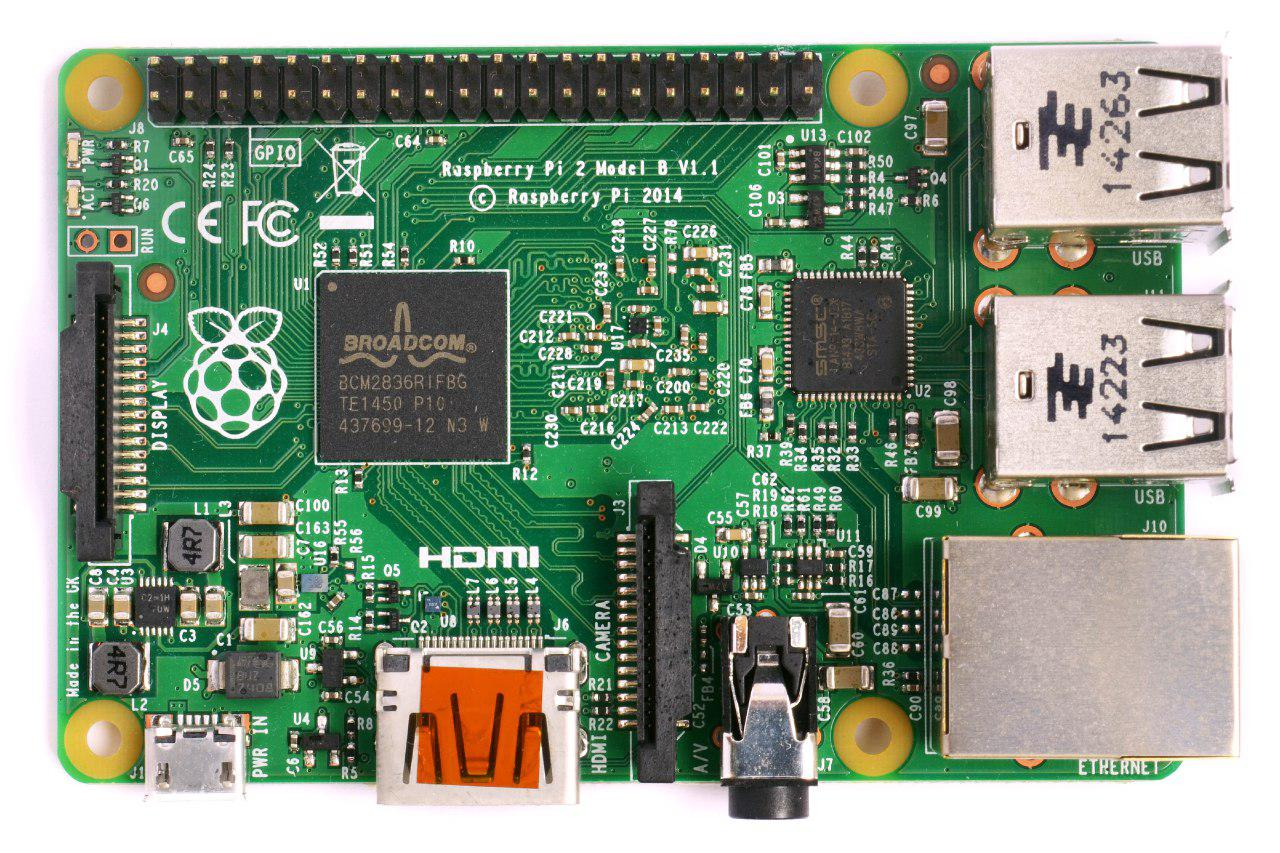
\includegraphics[height=5cm]{figures/Raspberry_Pi.jpg}
		\caption{Raspberry Pi Modelo 2b}
	\end{center}
	
	\label{rasp}
\end{figure}

Raspberry proporciona el sistema operativo oficial llamado Raspbian, una distribución de Debian. También soporta otros sistemas operativos.
 
Fue creado en 2006, en la Universidad de Cambridge, con el fin de fomentar la enseñanza en las escuela de ciencias de la computación, pero hasta 2012 no salió al mercado.

Existen distintos modelos de Raspberry Pi, desde la Raspberry Pi 1 Modelo A hasta la Raspberry Pi 3 Modelo B \ref{types}.
En nuestro proyecto hemos usado una Raspberry Pi 3 modelo B, con su sistema operativo oficial, Raspbian.

Se ha decidido utilizar este microcontrolador en el proyecto debido a su facilidad de manejo gracias a que cuenta con un sistema operativo y por ser relativamente barato para realizar un prototipo. Además cuenta con un gran comunidad detrás que trabaja en el desarrollo de nuevas guías y librerías para facilitar el desarrollo. 

\begin{figure}[htb]
	\begin{center}
		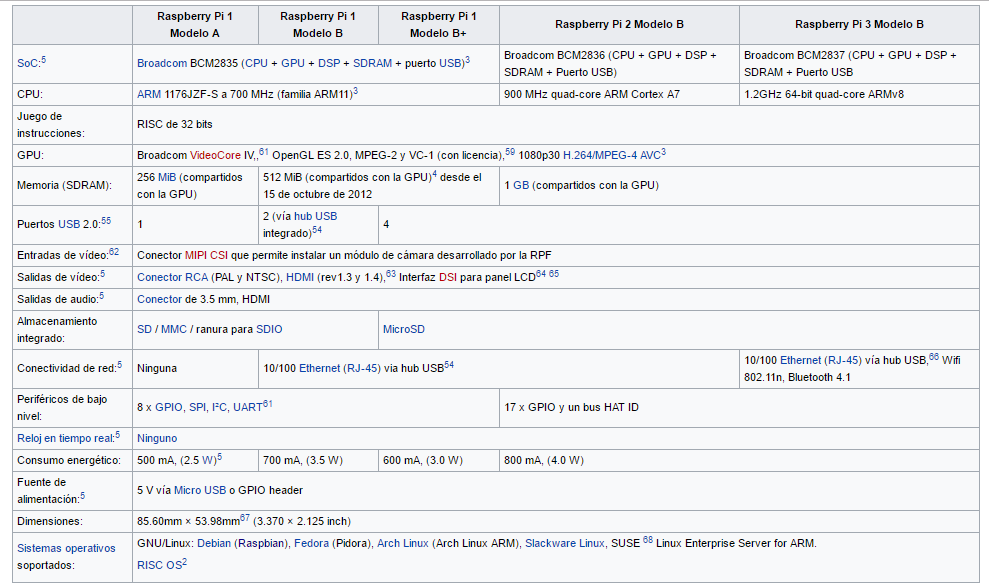
\includegraphics[width=17cm,height=12cm]{figures/Cuadro_Tipos_Raspberry.png}
		\caption{Cuadro comparativo de las especificaciones técnicas}
	\end{center}

	\label{types}
\end{figure}

\subsection{Sensor de temperatura y humedad}
\label{makereference2.3.2}

A la Raspberry se le conectan dos sensores, uno de temperatura y humedad y un piranómetro del cual hablaremos más tarde. Ambos para recoger los datos meteorológicos que necesitamos para nuestro modelo.

Para medir la temperatura y la humedad hemos utilizado un solo componente que recoge ambas muestras. El modelo escogido ha sido el sensor \textbf{DHT22}.

Algunas de las características de este sensor y en especial de este modelo (ya que tambien existe el modelo DHT11 de la misma marca) son que tiene una precisión de 0.5ºC para medir la temperatura, y entre un 2 y un 5 por ciento para la humedad. Ademas recogen dos muestras por segundo. Este sensor no es un sensor de alta precisión, pero es suficiente para nuestro proyecto, además de tener un precio muy económico. Ver imágen \ref{sensor}.

La comunicación entre el sensor y la Raspberry se realiza a través de un pin \textbf{GPIO} (General Purpose Input/Output, Entrada/Salida de Propósito General) que es un pin de propósito general. Estos pines pueden ser de entrada o de salida, y reciben y envían valores binarios de un bit.

En el \href{https://cdn-shop.adafruit.com/datasheets/Digital+humidity+and+temperature+sensor+AM2302.pdf}{datasheet} del sensor viene definido el proceso de comunicación entre este y la Raspberry. Para ello, el microcontrolador (Raspberry en nuestro caso) envía una señal de arranque para que el sensor cambie del estado ``standby'' al estado ``running''. Al terminar de enviar dicha señal, el sensor envía una respuesta de 40 bits que contiene la información relativa a la humedad (16 bits), a la temperatura (16 bits) y un checksum (8 bits) para comprobar que se ha enviado correctamente. Ver imagen \ref{DHT22comunication}.

El envío de estos bits sucede de la siguiente forma: el sensor envía una señal ``baja'' ("0") que indica el inicio de la transmisión de un bit. Seguidamente envía una señal ``alta'' (``1''). Si la transmisión de esta corriente dura más de $ 50 \mu $ s indica que se ha transmitido un 1, en caso contrario, se quiso transmitir un 0.

\begin{figure}[htb]
	
	\begin{center}
		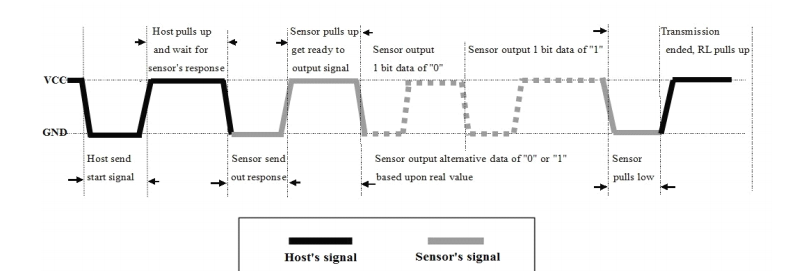
\includegraphics[width=15cm]{figures/DTH22comunicationdiagram.png}
		\caption{Diagrama de comunicación del sensor DHT22}
	\end{center}
	
	\label{DHT22comunication}
\end{figure} 

 \begin{figure}[htb]
	
	\begin{center}
		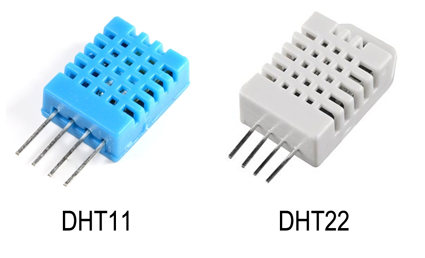
\includegraphics[width=7cm,height=7cm]{figures/sensorTemperaturaHumedad.png}
		\caption{Sensores de temperatura y humedad DHT11 y DHT22}
	\end{center}
	
	\label{sensor}
\end{figure} 

\subsection{Piranómetro y ADC}
\label{makereference2.3.3}
Para recoger la cantidad de irradiación solar se utiliza un piranómetro. En este proyecto se ha utilizado el modelo \href{https://www.apogeeinstruments.co.uk/content/SP-212-215-manual.pdf}{SP-212}. Este sensor es analógico es decir, la señal que envía es un voltaje variable con el cual indica la cantidad de irradiación que recoge.

Para poder leer esa información con un microcontrolador es necesario hacer una conversión a digital. Para ello se utiliza un conversor analógico-digital o por sus siglas en inglés \textbf{ADC}.

El \textbf{ADC} utilizado en este proyecto ha sido el \href{https://cdn-shop.adafruit.com/datasheets/MCP3008.pdf}{MCP3008}. Es un conversor de 10 bits por lo que permite codificar entre 0 y 1024, suficiente para este proyecto. Se comunica con la Raspberry a través del puerto \textbf{SPI}.

\textbf{SPI} es un estándar de comunicación en serie, maestro/esclavo, regulado por un reloj. Incluye 4 señales: reloj (SCLK), salida de datos del maestro y entrada de datos al esclavo (MOSI), salida de datos del esclavo y entrada al maestro (MISO) y otra para Para seleccionar un esclavo, o para que el maestro le diga al esclavo que se active (SS/Select).

Con cada pulso de reloj el maestro envía un bit. Para que empiece la transmisión el Master baja la señal SS/Select a cero, con esto el Slave se activa y empieza la transmisión, con un pulso de reloj al mismo tiempo que el primer bit es leído.

Raspberry cuenta con unos pines para la comunicación a través de SPI lo que facilita el uso de este tipo de componentes.

\section{Componentes software y librerías externas}
\label{makereference2.4}
El software a través del cual controlar el nodo ha sido escrito en Python2.7. Su punto de entrada es el archivo solar\_node.py.

Se puede ejecutar a través de la consola de comandos con el comando ``python solar\_node.py'' y para obtener la ayuda del comando ``python solar\_node.py -h''

Este programa tiene dos partes importantes: recoger los datos y enviarlos al servidor de datos. Para ello utilizamos varias librerías ya existentes.

\begin{itemize}  
\item \textbf{Adafruit\_DHT:} librería proporcionada por \href{https://www.adafruit.com/}{Adafruit} para leer e interpretar los datos proporcionados por el sensor DHT22. \textbf{Adafruit} es una compañía de hardware open-source, que además de proporcionar \textbf{hardware}, suministra de una gran cantidad de documentación y librerías para facilitar el trabajo con sus componentes. 
\item \textbf{Adafruit\_GPIO:} aporta la funcionalidad para acceder a los pines GPIO a través de python.
\item \textbf{Adafruit\_MCP3008:} comunicación a través de SPI con el ADC
\item \textbf{paho-mqtt:} Paho ha sido creado para proporcionar implementaciones escalables de código abierto de \textbf{protocolos de mensajería} abiertos y estándar dirigidos a aplicaciones nuevas, existentes y emergentes para Machine to Machine (M2M) e Internet of Things (IoT). Esta librería proporciona la funcionalidad para la comunicación a través de MQTT. Este protocolo de comunicación será exlicado más adelante.
\end{itemize}

\begin{figure}[htb]
	
	\begin{center}
		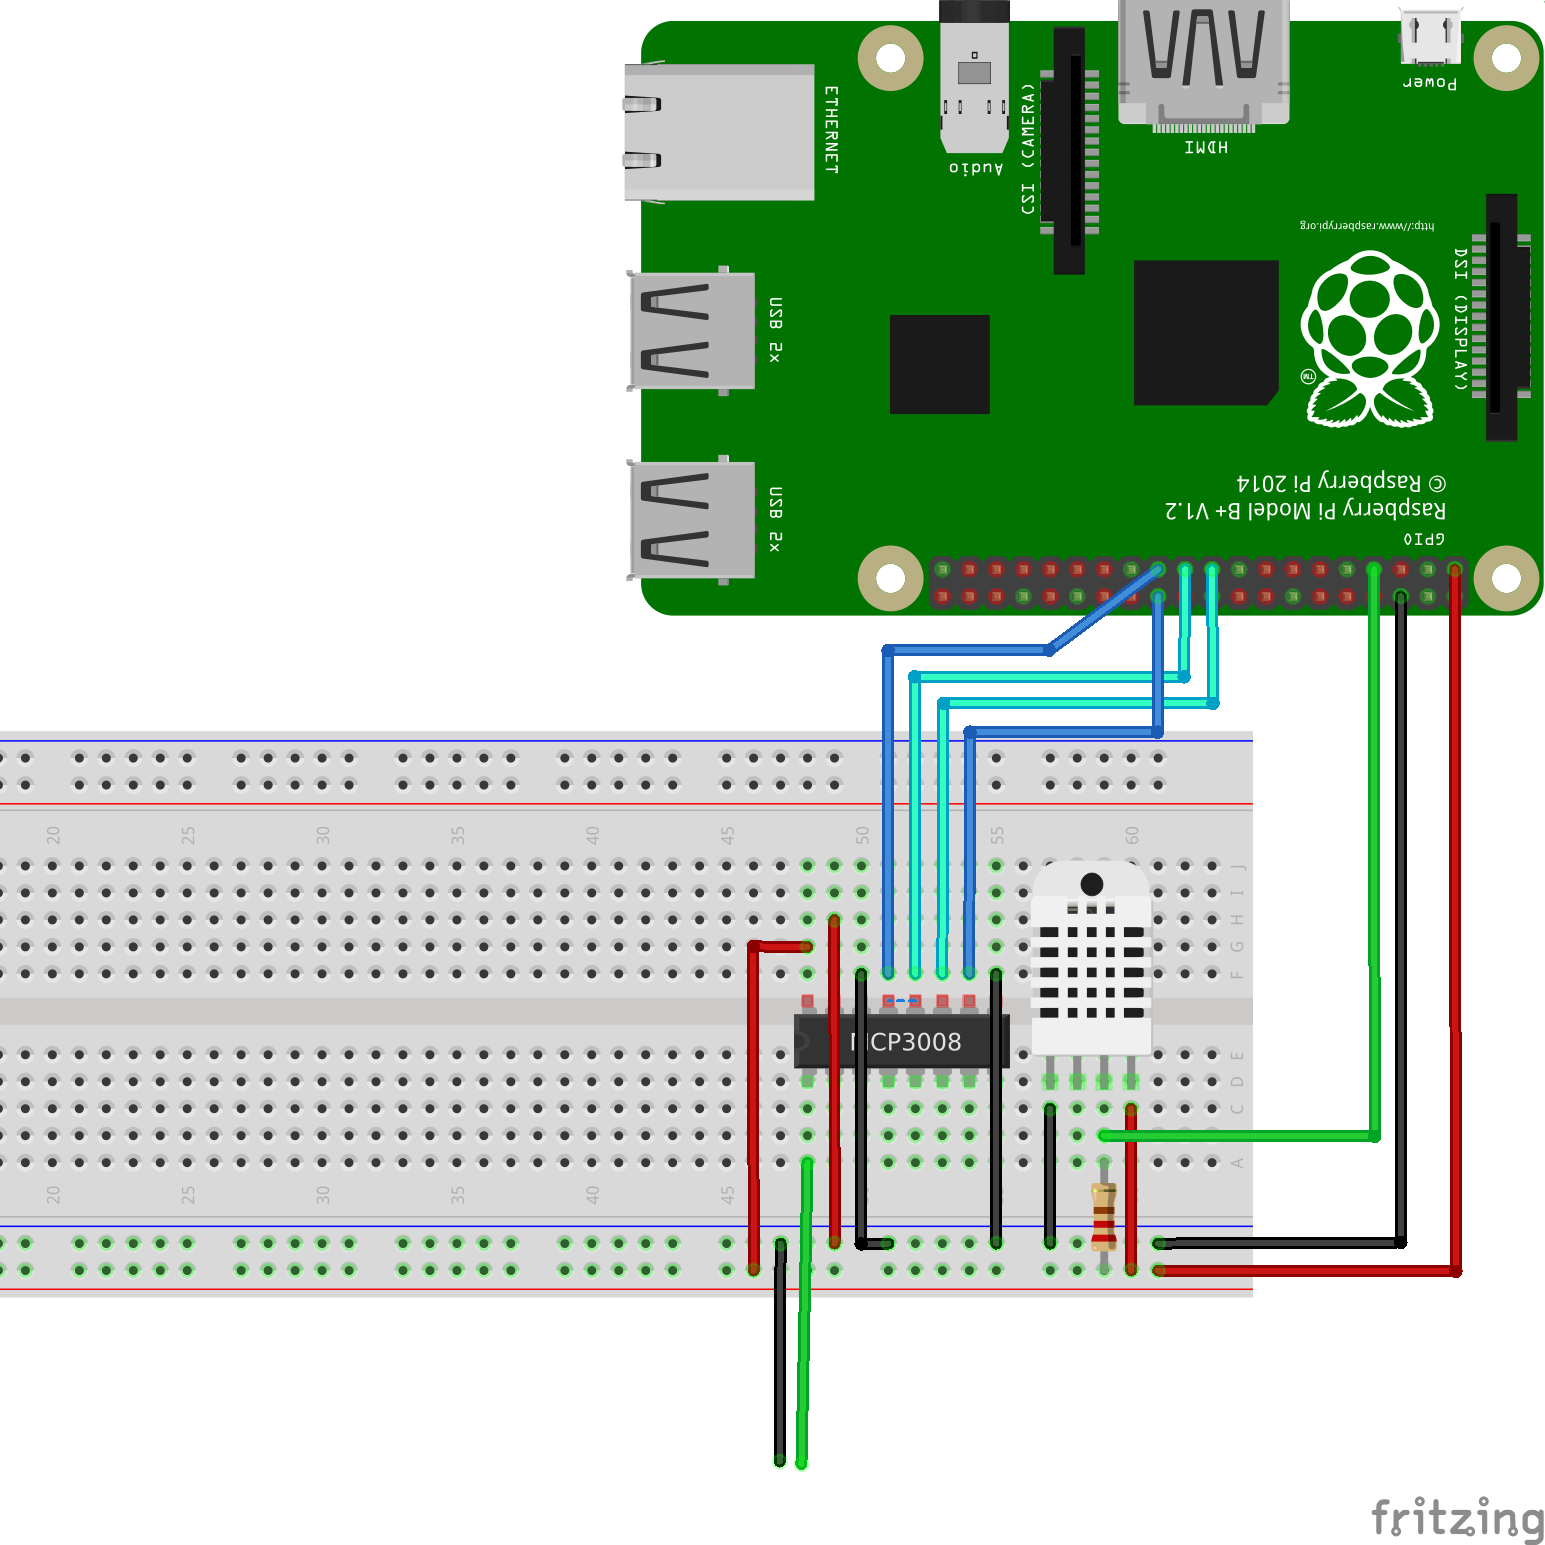
\includegraphics[width=15cm,height=15cm]{figures/solar_project_node_diagram.png}
		\caption{Diagrama del nodo}
	\end{center}
	
	\label{node-diagram}
\end{figure}
\cleardoublepage

\chapter{Exploración del modelo predictivo}
\label{makereference3}

Here are more examples of referring to previous sections.  In
Chapter~\ref{makereference} there were several sections, including
section~\ref{makereference1.1}, section~\ref{makereference1.2},
and section~\ref{makereference1.3}.

Likewise, in Chapter~\ref{makereference2}, there are
sections~\ref{makereference2.1} and ~\ref{makereference2.2}.

\section{Introducción a los modelos predictivos}
\label{makereference3.1}

Cuando hablamos de modelos predictivos nos estamos refiriendo al análisis que agrupa una serie de técnicas para conseguir analizar datos reales tanto actuales como históricos y así conseguir predicciones. Con esta predicción podremos saber cuanto se acerca nuestra predicción a la realidad.

\section{Descripción de las librerías usadas}
\label{makereference3.2}
	\subsection{Scikit-learn}
	Scikit-learn es una biblioteca de aprendizaje de software libre para el lenguaje de programación Python. Cuenta con varios algoritmos de clasificación, regresión y agrupación, incluyendo máquinas de vector de apoyo, bosques aleatorios, aumento de gradiente, k-medios y DBSCAN, y está diseñado para interoperar con las bibliotecas numéricas y científicas Python NumPy y SciPy.
	
	\subsection{NumPy}
	NumPy es una extensión de Python, que le agrega mayor soporte para vectores y matrices, constituyendo una biblioteca de funciones matemáticas de alto nivel para operar con esos vectores o matrices.
	
	\subsection{SciPy}
	SciPy es una biblioteca open source de herramientas y algoritmos matemáticos para Python. SciPy contiene módulos para optimización, álgebra lineal, integración, interpolación, funciones especiales, FFT, procesamiento de señales y de imagen, resolución de ODEs y otras tareas para la ciencia e ingeniería.
	
\section{Algoritmos utilizados}
\label{makereference3.3}
	\subsection{Regresión}
	
	\begin{figure}[htb]
		
		\begin{center}
			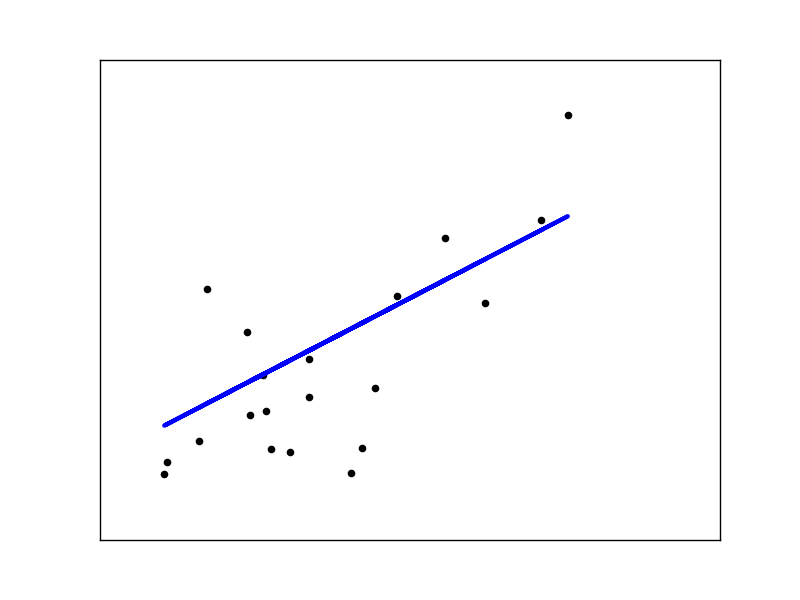
\includegraphics[height=3.5in]{figures/regression.png}
			\caption{Regresión lineal}
		\end{center}
		
		\label{regression}
	\end{figure}

	La \textbf{regresión lineal} es un modelo matemático que trata de hallar la \textbf{función lineal} que mejor se ajusta a un conjunto de puntos dispersos conocidos.
	
	Al conocer dicha función lineal, podremos \textbf{'predecir'} con un cierto grado de exactitud, lo que pasará.
	
	La línea recta que se puede ver en la gráfica \ref{regression}, muestra cómo la \textbf{regresión lineal} intenta dibujar una línea recta que minimice mejor la suma residual de cuadrados entre las respuestas observadas en el conjunto de datos, y las respuestas predichas por la aproximación lineal.
	También se calculan los coeficientes, la suma residual de cuadrados y el puntaje de varianza.
	
	\subsection{Clasificación}
	El término \textbf{clasificador} se utiliza en referencia al algoritmo utilizado para asignar un elemento entrante no etiquetado en una categoría concreta conocida. Dicho algoritmo, permite pues, ordenar o disponer por clases elementos entrantes, a partir de cierta información característica de estos.
	
	\subsection{Redes Neuronales}
	
	\begin{figure}[htb]
		
		\begin{center}
			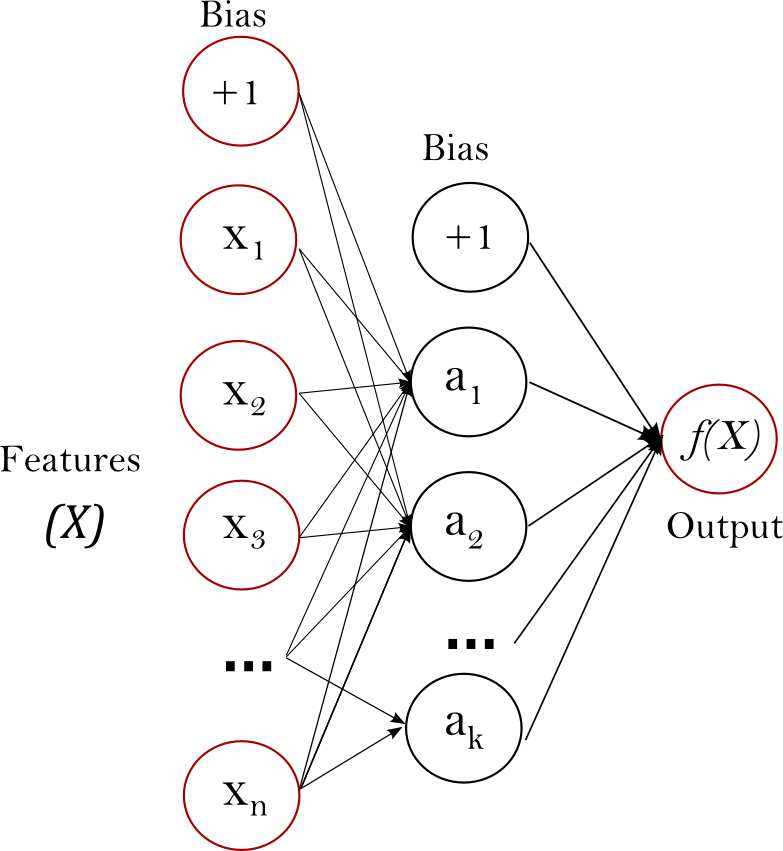
\includegraphics[height=4.5in]{figures/neuronal_network.png}
			\caption{Red neuronal}
		\end{center}
		
		\label{network}
	\end{figure}

	Las \textbf{redes neuronales} son un algoritmo de aprendizaje supervisado. Suelen consistir en varias capas ocultas donde la señal se propaga de adelante hacia atrás.
	
	A partir de X características se obtiene una función f(X).
	
\section{Protocolo del estudio}
\label{makereference3.4}

\section{Modelo escogido}
\label{makereference3.5}
\cleardoublepage

\chapter{Exploración del modelo predictivo}
\label{makereference4}

\section{Introducción a los modelos predictivos}
\label{makereference4.1}

 `` Cada día la gente se enfrenta a preguntas como: ¿Qué ruta debo tomar? ¿Debo cambiar de compañía telefónica? ¿Debo invertir mi dinero?
 
Lo que se quiere es conocer eventos futuros y sobre todo, conocerlos lo mejor posible.

La mayor parte de las veces se toma decisiones basándonos en información, pero muchas otras nos guiamos por nuestra intuición o la propia experiencia.

Pero de todas maneras se está prediciendo a partir de la información y experiencia que tenemos y tomando decisiones a partir de estas predicciones. '' 


Cuando hablamos de modelos predictivos nos estamos refiriendo al análisis que agrupa una serie de técnicas para conseguir analizar datos reales tanto actuales como históricos y así conseguir predicciones. Con esta predicción podremos saber cuanto se acerca nuestra predicción a la realidad.

 

\section{Descripción de las librerías usadas}
\label{makereference4.2}
	\subsection{Scikit-learn}
	\label{makereference4.2.1}
	Scikit-learn es una biblioteca de aprendizaje de software libre para el lenguaje de programación Python. Cuenta con varios algoritmos de clasificación, regresión y agrupación, incluyendo máquinas de vector de apoyo, bosques aleatorios, aumento de gradiente, k-medios y DBSCAN, y está diseñado para interoperar con las bibliotecas numéricas y científicas Python NumPy y SciPy. (\cite{ARP:Scikit:2017})
	
	\subsection{NumPy}
	\label{makereference4.2.2}
	NumPy es una extensión de Python, que le agrega mayor soporte para vectores y matrices, constituyendo una biblioteca de funciones matemáticas de alto nivel para operar con esos vectores o matrices. (\cite{ARP:Numpy:2017})
	
	\subsection{SciPy}
	\label{makereference4.2.3}
	SciPy es una biblioteca open source de herramientas y algoritmos matemáticos para Python. SciPy contiene módulos para optimización, álgebra lineal, integración, interpolación, funciones especiales, FFT, procesamiento de señales y de imagen, resolución de ODEs y otras tareas para la ciencia e ingeniería. (\cite{ARP:Scipy:2017})
	
\section{Algoritmos utilizados}
\label{makereference4.3}
	\subsection{Regresión}
	\label{makereference4.3.1}
	\begin{figure}[htb]
		
		\begin{center}
			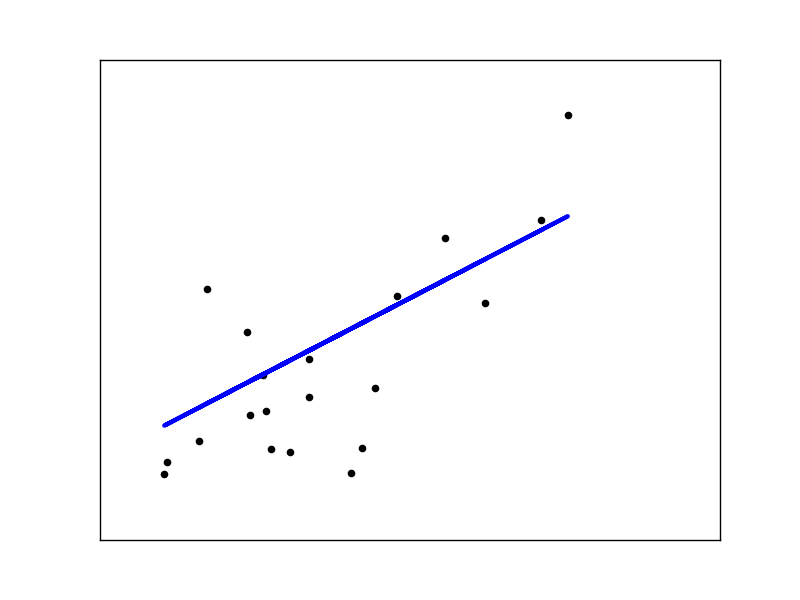
\includegraphics[height=3.5in]{figures/regression.png}
			\caption{Regresión lineal [Fuente: \href{www.wikipedia.org}{Wikipedia}]}
		\end{center}
		
		\label{regression}
	\end{figure}

	La \textbf{regresión lineal} es un modelo matemático que trata de hallar la \textbf{función lineal} que mejor se ajusta a un conjunto de puntos dispersos conocidos.
	
	Al conocer dicha función lineal, podremos \textbf{'predecir'} con un cierto grado de exactitud, lo que pasará.
	
	La línea recta que se puede ver en la gráfica \ref{regression}, muestra cómo la \textbf{regresión lineal} intenta dibujar una línea recta que minimice mejor la suma residual de cuadrados entre las respuestas observadas en el conjunto de datos, y las respuestas predichas por la aproximación lineal.
	También se calculan los coeficientes, la suma residual de cuadrados y el puntaje de varianza.
	
	\subsection{Clasificación}
	\label{makereference4.3.2}
	El término \textbf{clasificador} se utiliza en referencia al algoritmo utilizado para asignar un elemento entrante no etiquetado en una categoría concreta conocida. Dicho algoritmo, permite pues, ordenar o disponer por clases elementos entrantes, a partir de cierta información característica de estos.
	
	\subsection{Redes Neuronales}
	\label{makereference4.3.3}
	
	\begin{figure}[htb]
		
		\begin{center}
			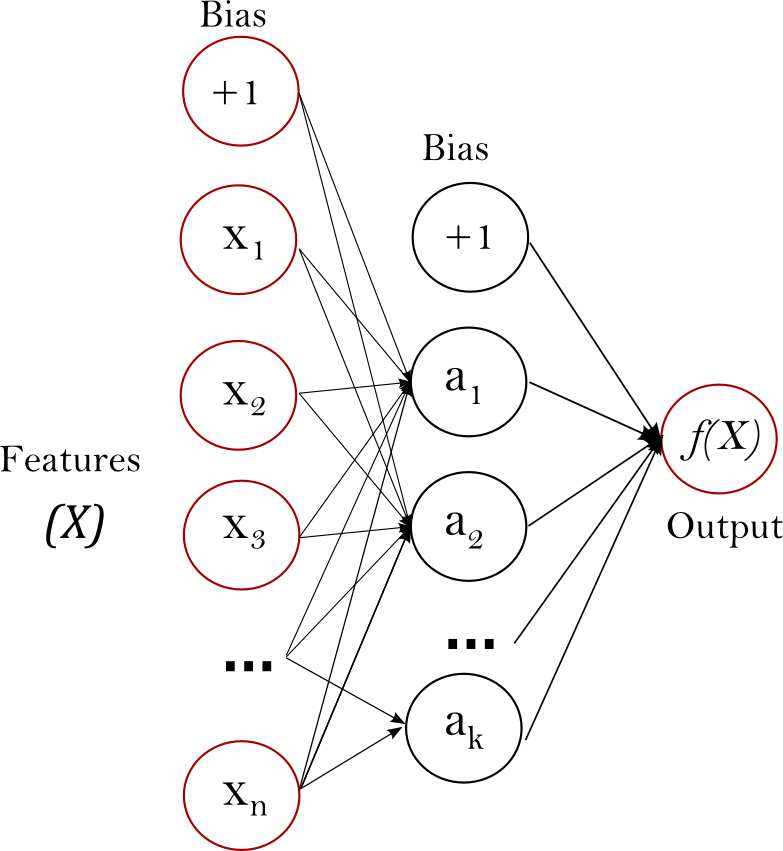
\includegraphics[height=4.5in]{figures/neuronal_network.png}
			\caption{Red neuronal [Fuente: \href{www.scikit-learn.org}{scikit-learn}]}
		\end{center}
		
		\label{network}
	\end{figure}

	Las \textbf{redes neuronales} son un algoritmo de aprendizaje supervisado. Suelen consistir en varias capas ocultas donde la señal se propaga de adelante hacia atrás.
	
	A partir de X características se obtiene una función f(X).
	
\section{Protocolo del estudio}
\label{makereference4.4}

\section{Modelo escogido}
\label{makereference4.5}
\cleardoublepage

\chapter{Servidor de datos}
\label{makereference5}

Here are more examples of referring to previous sections.  In
Chapter~\ref{makereference} there were several sections, including
section~\ref{makereference1.1}, section~\ref{makereference1.2},
and section~\ref{makereference1.3}.

Likewise, in Chapter~\ref{makereference2}, there are
sections~\ref{makereference2.1} and ~\ref{makereference2.2}.

\section{Introducción}
\label{makereference5.1}
Como comentamos en el capitulo anterior, el \textbf{nodo} necesita una interfaz de red para mandar los datos, en este caso estamos hablando de \textbf{MQTT}. Este sera el encargado de recibir, almacenar y organizar la información que recibe del nodo.
El \textbf{cliente MQTT} lo ejecuta el nodo y por otro lado el \textbf{servidor MQTT} esta en una máquina física que hemos alojado en la Facultad de Físicas, a la cual accedemos por SSH remotamente.

\section{MQTT}
\label{makereference5.2}
\textbf{MQTT} o lo que es lo mismo \textit{Message Queue Telemetry Transpor}t es un protocolo para la comunicación \textbf{machine-to-machine} de mensajería bastante simple y ligero, orientado a conexión por \textbf{TCP/IP}. Esta diseñado principalmente para dispositivos con poco ancho de banda y con latencia baja. 

Tiene dos puertos TCP/IP reservados, el 1883 y el 8883.

\section{ThingSpeak}
\label{makereference5.3}

\section{Bridge ThingSpeak}
\label{makereference5.4}

\section{Instalación y puesta en marcha}
\label{makereference5.5}
\cleardoublepage

\chapter{Resultados}
\label{makereference6}

\section{Entrenamiento}
\label{makereference6.1}

\section{ThinkSpeak}
\label{makereference6.2}

\section{Calidad del código}
\label{makereference6.3}

\begin{figure}[htb]
	Una vez acabado el código del proyecto, decidimos certificar su calidad mediante \textbf{codacy}.
	\textbf{Codacy} es una herramienta que proporciona nuestro controlador de versiones \textbf{GitHub}. Sencillamente revisa todas y cada una de las líneas del código, para hacerlo más sencillo, escalable y seguro. Genera un informe con los errores y te dice qué grado de calidad tiene, siendo A el más alto. (\cite{ARP:Codacy:2017})
	
	\begin{center}
		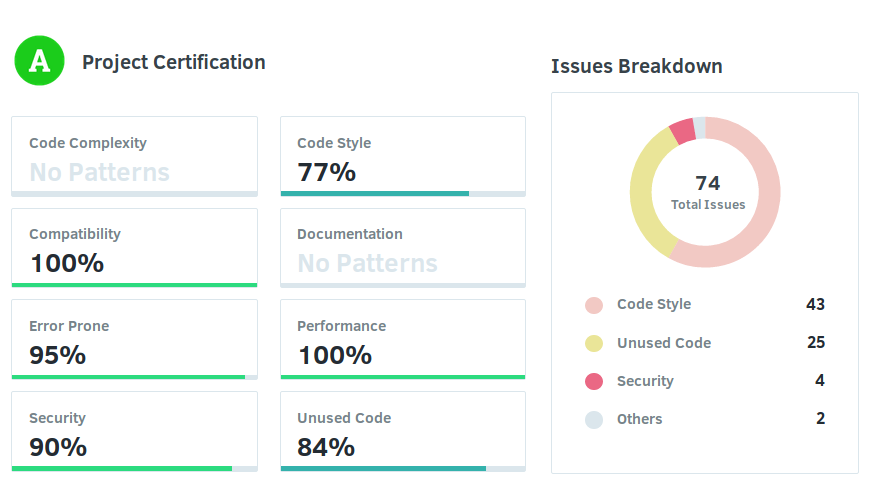
\includegraphics[height=3.5in]{figures/codacy.png}
		\caption{Informe de nuestro proyecto [Fuente: \href{https://www.codacy.com}{Codacy}]}
	\end{center}
	
	\label{codacy}
\end{figure}
\cleardoublepage

\chapter{Instalación y puesta en marcha}
\label{makereference7}

Para poner en funcionamiento el proyecto deberemos tener todos lo elementos que lo componen:
\begin{itemize}
\item Nodo.
\item Servidor de datos.
\item Servidor de cálculo. Puede estar alojado en la misma máquina que el servidor de datos.
\item Sistema de visualización. En este caso, estar registrado en ThingSpeak y tener una clave de aplicación.
\end{itemize}

\section{Nodo}
\label{makereference7.1}
\subsection{Requisitos}
\label{makereference7.1.2}
	\begin{itemize}
		\item \textbf{Raspberry Pi 3 model B} con una distribución Linux (\href{https://www.raspberrypi.org/downloads/raspbian/}{Raspbian}).
		\item Conexión a Internet.
		\item \href{https://www.adafruit.com/product/385}{Sensor DHT22}.
		\item Conversor analógico-digital \href{https://www.adafruit.com/product/856}{MCP3008}.
		\item Piranómetro \href{https://www.apogeeinstruments.co.uk/content/SP-212-215-manual.pdf}{SP-212}.
		\item SPI activo en la Raspberry con ``raspi-config''.
	\end{itemize}

El cableado de los componentes HW está descrito en la figura \ref{wiring}.
\begin{figure}[htb]
	\begin{center}
		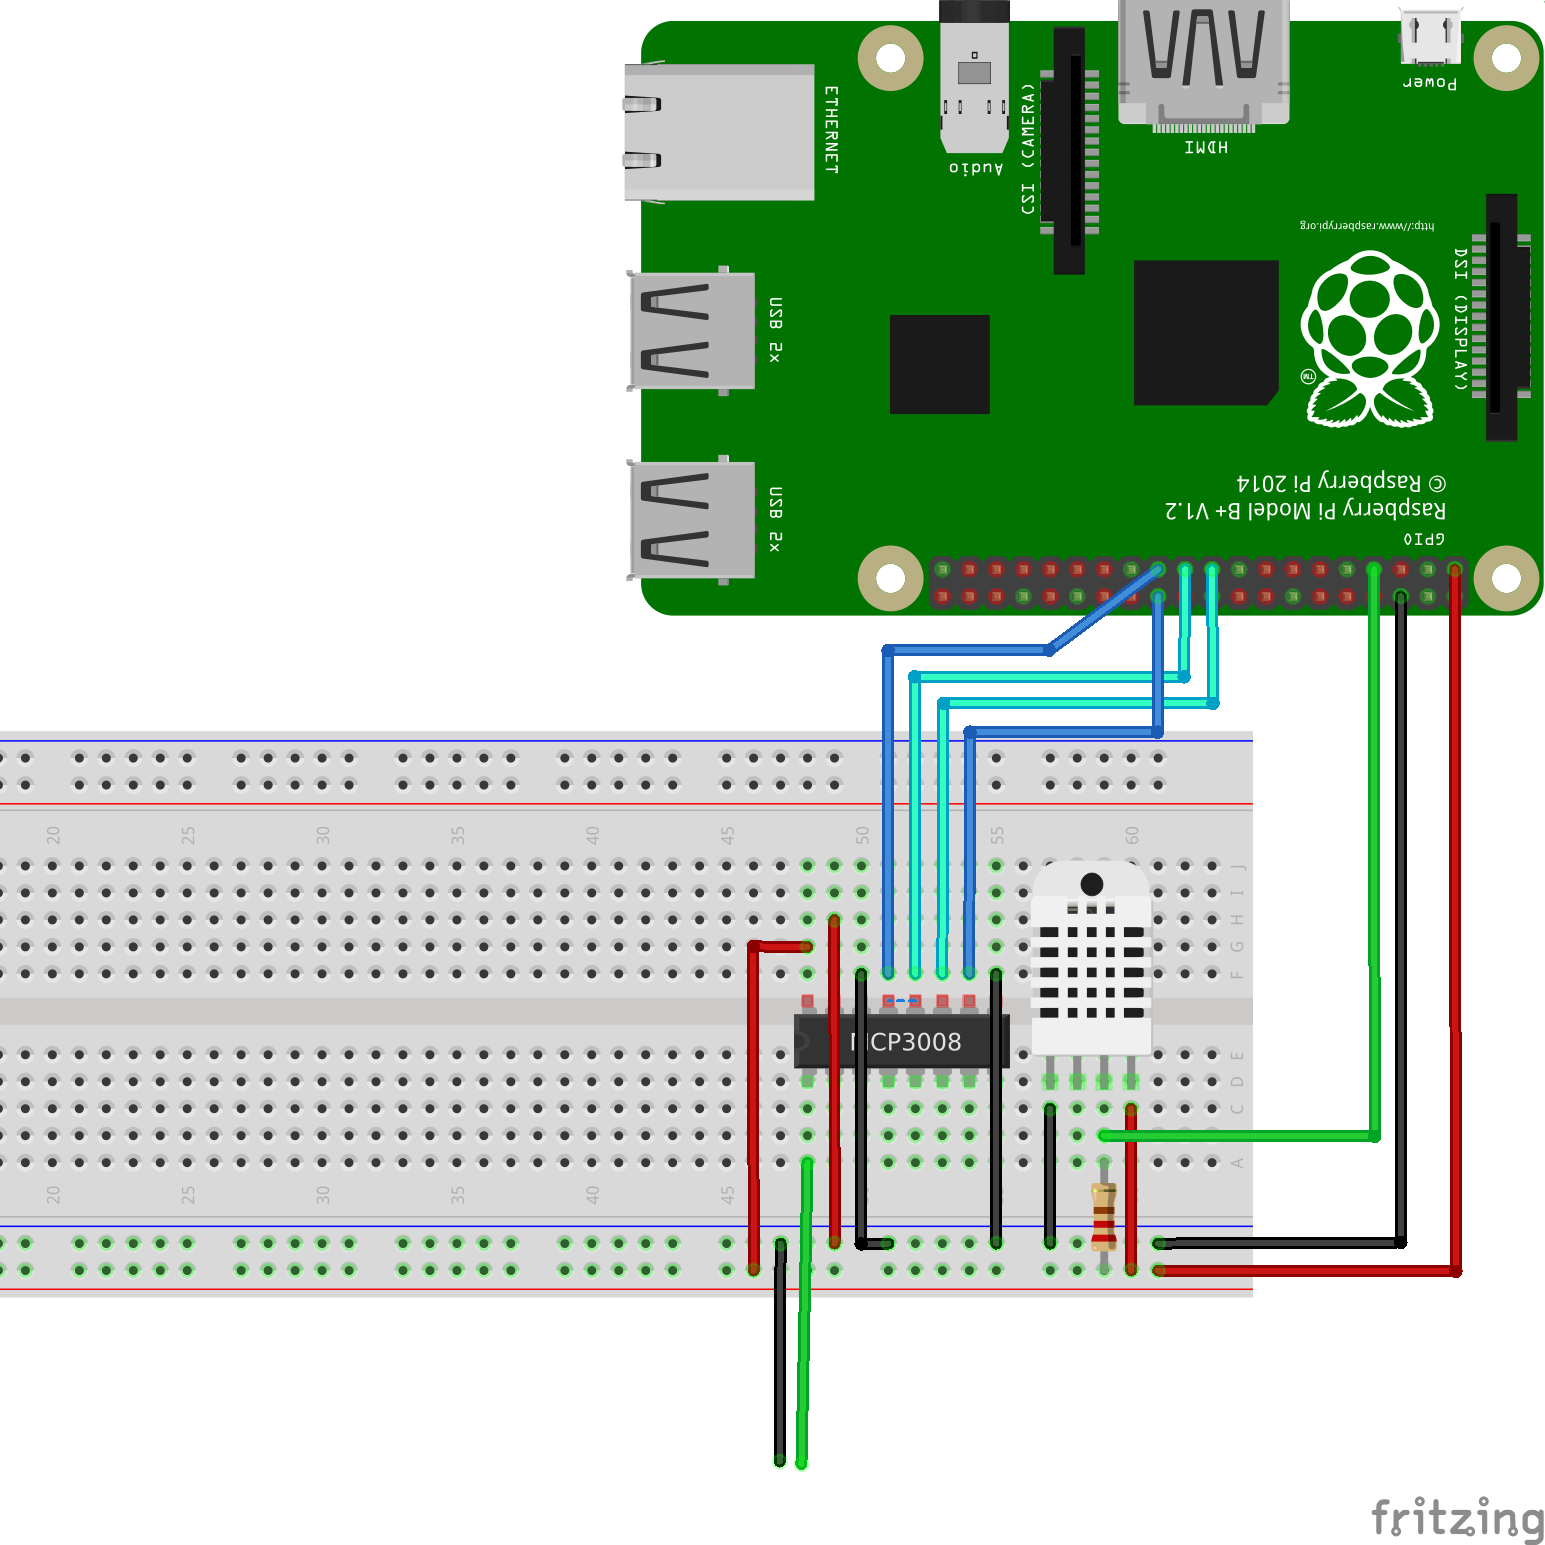
\includegraphics[width=12cm]{figures/solar_project_node_diagram.png}
		\caption{Cableado del nodo}
	\end{center}

Por defecto, Ubuntu arranca el servicio después de instalarlo. Si la distribución Lunix sobre la cual se instala no realiza esta acción por defecto, se deberá configurar debidamente para arrancarlo.

En este proyecto se utiliza la configuración por defecto de Mosquitto. Para más información sobre su configuración, consultar \href{https://www.digitalocean.com/community/tutorials/how-to-install-and-secure-the-mosquitto-mqtt-messaging-broker-on-ubuntu-16-04}{más información}.

	\label{wiring}
\end{figure}

\subsection{Ficheros}
\label{makereference7.1.3}
Los archivos necesarios para la instalación del software del nodo se encuentran disponibles en \href{https://github.com/MrSlide22/TFG/node}{Github}.

\begin{itemize}
	\item Introduce el directorio \textbf{node} en tu Rapsberry Pi
	\item Cambia las variables \textbf{brokerIp, brokerPort, topic, ubication} en solar\_node.py
\end{itemize}

\subsection{Dependencias}
\label{makereference7.1.4}
	\begin{itemize}
		\item Actualizar
\lstset{language=bash}
\begin{lstlisting}[frame=single]
$ sudo apt-get update
$ sudo apt-get upgrade
\end{lstlisting}
		\item Python 2.7 (\cite{ARP:Python:2017})
\begin{lstlisting}[frame=single]
$ sudo apt-get install python2.7 build-essential 
python-pip python-dev
\end{lstlisting}
		\item Paho (\cite{ARP:Paho:2017})
\begin{lstlisting}[frame=single]
$ pip install paho-mqtt
\end{lstlisting}
		\item WiringPi (\cite{ARP:Wiring:2017})
\begin{lstlisting}[frame=single]
$ pip install wiringpi2
\end{lstlisting}
		\item Adafruit\_DHT (\cite{ARP:Adafruit:2017})
\begin{lstlisting}[frame=single]
$ git clone 
https://github.com/adafruit/Adafruit_Python_DHT.git
$ cd Adafruit_Python_DHT
$ sudo python setup.py install
\end{lstlisting}
		\item Adafruit\_GPIO
\begin{lstlisting}[frame=single]
$ git clone 
https://github.com/adafruit/Adafruit_Python_GPIO.git
$ cd Adafruit_Python_GPIO
$ sudo python setup.py install
\end{lstlisting}
		\item Adafruit\_MCP3008
\begin{lstlisting}[frame=single]
$ git clone 
https://github.com/adafruit/Adafruit_Python_MCP3008.git
$ cd Adafruit_Python_MCP3008
$ sudo python setup.py install
\end{lstlisting}
	\end{itemize}

\subsection{Puesta en marcha del nodo}
\label{makereference7.1.5}
Para arrancar el nodo se deberá haber seguido todos los pasos anteriores. Posteriormente, desde un terminal de la Raspberry, ir a la carpeta donde se han guardado el código fuente y ejecutar el comando: 

\lstset{language=bash}
\begin{lstlisting}[frame=single]
$ sudo python solar_node.py
\end{lstlisting}

Se debe ser superusuario para poder ejecutar este comando.

% TODO - referenciar "descripción del nodo" de la línea de abajo
Para obtener más información sobre cómo utilizar el nodo ver Descripción del nodo o ejecutar:

\lstset{language=bash}
\begin{lstlisting}[frame=single]
$ sudo python solar_node.py -h
\end{lstlisting}

\section{Servidor de datos}
\label{makereference7.2}
\subsection{Requisitos previos}
\label{makereference7.3}
\begin{itemize}
\item Máquina con distribucion Linux instalada. Recomendable Debian, Fedora, OpenSUSE o Ubuntu.
\item conexión a internet.
\item IP fija y opcionalmente, nombre de dominio.
\end{itemize}

La instalación de un broker MQTT es muy sencilla (una de sus principales ventajas). Para ello basta con instalar el demonio mosquitto a través del siguiente comando:

Ejemplo de instalación en Ubuntu:
\lstset{language=bash}
\begin{lstlisting}[frame=single]
$ sudo apt-get install mosquitto
\end{lstlisting}

Por defecto, Ubuntu arranca el servicio después de instalarlo. Si la distribución Lunix sobre la cual se instala no realiza esta acción por defecto, se deberá configurar debidamente para arrancarlo.

En este proyecto se utiliza la configuración por defecto de Mosquitto. Para más información sobre su configuración, consultar \href{https://www.digitalocean.com/community/tutorials/how-to-install-and-secure-the-mosquitto-mqtt-messaging-broker-on-ubuntu-16-04}{más información}.

\section{Servidor de cálculo}
\label{makereference7.3}

\subsection{Requisitos previos}
\label{makereference7.3.1}

\begin{itemize}
\item Máquina con distribución Linux.
\item Python 2.7.
\item Conexión a internet.
\item IP fija y opcionalmente, nombre de dominio.
\end{itemize}

\subsection{Instalación}
\label{makereference7.3.2}
Los archivos necesarios para la instalación del software del servidor de cálculo se encuentran disponibles en \href{https://github.com/MrSlide22/TFG/server}{Github}.

\begin{itemize}
	\item Introduce el directorio \textbf{server} en el servidor.
	% TODO - revisar cuales son las variables necesarias
	\item Cambia las variables \textbf{ThingSpeakKey} en solar\_server.py
\end{itemize}

%\bibliographystyle{styles/plain}
\bibliographystyle{styles/plain}

%\bibdata{references}
\bibliography{references}
%\addcontentsline{toc}{chapter}{Bibliography}

\appendix
% +--------------------------------------------------------------------+
% | Appendix A Page (Optional)                                         |
% +--------------------------------------------------------------------+

\cleardoublepage

\chapter{Title for This Appendix}
\label{Appendix:Key1}


% +--------------------------------------------------------------------+
% | Enter text for your Appendix page in the space below this box.     |
% |                                                                    |
% +--------------------------------------------------------------------+

% +--------------------------------------------------------------------+
% | Appendix B Page (Optional)                                         |
% +--------------------------------------------------------------------+

\cleardoublepage

\chapter{Title for This Appendix}
\label{Appendix:Key2}

% +--------------------------------------------------------------------+
% | Enter text for your Appendix page in the space below this box.     |
% |                                                                    |
% +--------------------------------------------------------------------+


\end{document}
